\documentclass[../main.tex]{subfiles}
\begin{document}
\newpage
\thispagestyle{empty}
\begin{center}
    {
\includegraphics[width=0.5\textwidth]{Imagenes/Logo UMA.jpg}\par}
    \vspace{1cm}
    {\bfseries\LARGE \Facultad \par}
    \vspace{0.5cm}
    {\scshape\Large \Grado \par}
    \vspace{1.5cm}
    {\scshape\Huge Anexo I \par}
    \vspace{0.5cm}
    {\scshape\Huge Diseño de Instalación de Fontanería \par}
    \vspace{1.5cm}
    {\itshape\Large \TituloProyecto \par}
    \vfill
    {\Large Solicitante: \par}
    {\Large \Solicitante  \par}
    \vspace{1cm}
    {\Large Autores: \par}
    {\Large \Autora \par}
    {\Large \Autor \par}
    \vfill
    {\Large \Fecha \par}
\end{center}

\newpage
\section{Introducción}
En el diseño de la instalación de fontanería se tendrá en cuenta las dimensiones y la demanda de agua de la nave industrial así como el documento básico de salubridad del código técnico de la edificación y las normas y recomendaciones de la compañía suministradora, en este caso EMASA. \par
\vspace{0.5 cm}
En este anexo se detallan los cálculos llevados a cabo para su diseño así como los resultados y las consideraciones previas a ellos. Dicho diseño se ha llevado a cabo siguiendo el siguiente procedimiento:

\begin{enumerate}
    \item Realización de un croquis de la instalación.
    \item Definir recorrido principal o más desfavorable y delimitar cada tramo. Estimar la longitud de cada tramo incluidas las partes verticales.
    \item Obtener caudal instantáneo mínimo a partir de la tabla 2.1 de la sección HS 4 del Código Técnico de la Edificación.
    \item Obtener caudal total instalado como suma de los caudales instantáneos mínimos.
    \item Calcular el caudal simultáneo para cada tramo.
    \item Fijar un diámetro interior de la tubería y comprobar que la velocidad esté dentro de los márgenes fijador por el DB HS-4. 
    \item Hallar la pérdida unitaria de carga por rozamiento para cada tramo.
    \item Obtener la pérdida de carga total y determinar la presión de suministro necesaria para la instalación.
    \item En caso necesario diseñar un grupo de presión auxiliar.
\end{enumerate}

\section{Características de la nave a considerar}
Para el cálculo y dimensionamiento de la instalación de fontanería en la nave, se debe tener en cuenta la demanda de esta. Para ello se detallan a continuación la cantidad y tipo de aparatos a instalar y su localización. 
\begin{table}[H]
    \centering
    \begin{tabular}{c|c}
         Objeto & Cantidad \\ \hline
         Inodoro & 9 \\
         Lavabo & 5 
    \end{tabular}
    \caption{Instalación de fontanería planta baja.}
\end{table}

\begin{table}[H]
    \centering
    \begin{tabular}{c|c}
         Objeto & Cantidad \\ \hline
         Ducha & 8 \\
         Lavabo & 4 
    \end{tabular}
    \caption{Instalación de fontanería entreplanta.}
\end{table}

\section{Condiciones mínimas del suministro de agua}
Para el diseño de la instalación de fontanería se aplicará la normativa expuesta en el HS 4 sobre suministro de agua dentro del documento básico de salubridad del CTE. Esta será aplicable tanto para agua fría como para agua caliente sanitaria. Dichas condiciones mínimas son:

\begin{itemize}
    \item En los puntos de consumo la presión mínima debe ser de 100 kPa para grifos comunes y de 150 kPa para calentadores.
    \item La presión en cualquier punto de consumo no debe superar 500 kPa.
    \item La temperatura de ACS en los puntos de consumo debe estar comprendida entre 50ºC y 65ºC.
    \item La velocidad deberá ser de entre 0,50 y 2,00 m/s en tuberías metálicas, y de entre 0,50 y 3,50 m/s en tuberías termoplásticas y multicapas.
\end{itemize}

Se considera también un caudal mínimo que se tiene que suministrar a cada aparato según su tipo. Estos caudales se detallan en la tabla 2.1 del HS4. Para esta instalación en particular se consideran los siguientes caudales:

\begin{table}[H]
    \centering
    \begin{tabular}{c|c|c}
         Tipo de aparato & $Q_{min} [dm^3/s]$ & $Q_{min} ACS [dm^3/s]$ \\ \hline
         Lavabo & 0,10 & 0,065 \\
         Ducha & 0,20 & 0,10 \\
         Inodoro con cisterna & 0,10 & - \\
    \end{tabular}
    \caption{Caudal instantáneo mínimo para cada tipo de aparato.}
\end{table}

\section{Cálculos}
\subsection{Acometida}
Para el dimensionado de la acometida, se calcula en primer lugar el caudal total mínimo que se debe tener sen la instalación haciendo uso de la tabla previamente expuesta. Se obtiene así un caudal mínimo de $3,4 [dm^3/s]$.\par
\vspace{0.5 cm}
A este caudal obtenido se le aplicará un coeficiente de simultaneidad antes de usarlo para el cálculo de la instalación. Dicho coeficiente vendrá dado por la expresión:
\[K = \frac{1}{\sqrt{n - 1}}\]
Siendo:
\begin{itemize}
    \item n: número de aparatos en la red
    \item K: coeficiente de simultaneidad
\end{itemize}
Se obtiene así un coeficiente de simultaneidad de $K = 0,20$ decidiendo aumentarlo hasta $0,25$. Calculándose con este un caudal instantáneo de:
\[Q_{instantaneo} = Q_{instalado} \times K = 0,85 dm^3/s\]
Una vez calculado el caudal instantáneo se procede a la obtención del diámetro necesario en la acometida. Para ello se hace uso de la formula de Hazen-Williams:
\[D = \sqrt{\frac{Q \times 4}{\pi \times v}}\]
Donde:
\begin{itemize}
    \item Q: caudal instantáneo [$m^3/s$]
    \item v: velocidad del agua [$m/s$]
    \item D: diámetro de la acometida [$m$]
\end{itemize}
Teniendo en consideración el rango de velocidades de agua expuesto en el DB-HS 4, en este caso se decide utilizar tuberías de PVC para toda la instalación por lo que se deberá asegurar una velocidad de entre $0,50$ y $3,50$ m/s.Se decide usar una de $2,0 m/s$, que se encuentra comprendida en dicho rango. Así se obtiene un diámetro de acometida de $23,2621 mm$. Para usar un diámetro de tubo normalizado se utilizará uno de $25 mm$, con el cuál se obtiene una velocidad de agua aproximada de $1,7 m/s$, valor que se encuentra dentro del rango previamente mencionado. \par
\vspace{0.5 cm}
\textbf{Acometida de PVC de 25mm de diámetro.}

\subsection{Dimensionado de las tuberías de la instalación}
Para el diseño se seguirá el siguiente procedimiento:
\begin{itemize}
    \item Calcular el caudal total para cada tramo de la instalación y posteriormente el caudal simultáneo o de cálculo.
    \item Fijar diámetro de tuberías y comprobar que la velocidad a través del mismo está dentro de los márgenes indicados en el apartado 4.2.1. de la sección HS4 del CTE.
\end{itemize}

Se decide utilizar tuberías interiores de polietileno reticulado. Para los cálculos del dimensionamiento de las tuberías se hace uso de las mismas expresiones que para la acometida. A continuación de detallan los tramos de la instalación y los diámetros de tuberías calculados para dichos tramos.

\begin{table}[H]
    \centering
    \begin{tabular}{c | c | c | c}
         Tramos & Inodoros & Lavabos & Duchas \\ \hline
         1 & 9 & 9 & 8 \\ 
         2 & 4 & 2 & - \\ 
         3 & 1 & 1 & - \\ 
         4 & 4 & 2 & - \\ 
         5 & - & 2 & 4 \\ 
         6 & - & 2 & 4 \\ 
         7 & - & 9 & 8 \\
         8 & - & 5 & - \\ 
         9 & - & 2 & 4\\ 
         10 & - & 2 & 4 \\ 
    \end{tabular}
    \caption{Tramos de la instalación.}
\end{table}

\begin{table}[H]
    \centering
    \begin{tabular}{c | c | c | c | c | c | c | c | c}
         Tramo & $Q [l/s]$ & $K$ & $Q_c [l/s]$ & $v [m/s]$ & $D_{min} [mm]$ & $D_{int} [mm]$ & $D_{ext} [mm]$ & $v_{real} [m/s]$ \\ \hline
         1 & 3,4 & 0,20 & 0,68 & 1,7 & 22,5676 & 25 & 27 & 1,3853 \\
         2 & 0,60 & 0,4472 & 0,2683 & 1,7 & 14,1763 & 16 & 18 & 1,3344\\
         3 & 0,20 & 1 & 0,20 & 1,7 & 12,239 & 16 & 18 & 0,9947\\
         4 & 0,60 & 0,4472 & 0,2683 & 1,7 & 14,1763 & 16 & 18 & 1,3344 \\
         5 & 1 & 0,4472 & 0,4472 & 1,7 & 18,3016 & 20 & 22 & 1,4235 \\
         6 & 1 & 0,4472 & 0,4472 & 1,7 & 18,3016 & 20 & 22 & 1,4235\\
         7 & 1,3850 & 0,25 & 0,3463 & 1,7 & 16,1037 & 20 & 22 & 1,1023\\
         8 & 0,3250 & 0,50 & 0,1625 & 1,7 & 11,0321 & 16 & 18 & 0,8082\\
         9 & 0,53 & 0,4472 & 0,2370 & 1,7 & 13,3237 & 16 & 18 & 1,1787\\
         10 & 0,53 & 0,4472 & 0,2370 & 1,7 & 13,3237 & 16 & 18 & 1,1787\\
    \end{tabular}
    \caption{Resultados de cálculo.}
\end{table}

Se comprueba que todas las velocidades reales están dentro del rango que exige la norma.

\subsection{Pérdidas de carga}
Se comprobará que la presión disponible en el punto de consumo más desfavorable supera los valores mínimos indicados en el apartado 2.1.3 del CTE DB HS-4 y que no se supera el valor máximo indicado en el mismo apartado. \par
\vspace{0.5 cm}
Para ello se determinará la presión del circuito sumando las pérdidas de presión total de cada tramo, para ello se hará uso de la ecuación de Darcy-Weisbach. \par
\vspace{0.5 cm}
En primer lugar se calculará el número de Reynolds a partir de la siguiente expresión: \par
\[R_e = \frac{\rho \times D \times v}{\mu}\]
Donde:
\begin{itemize}
    \item $\rho$: densidad del fluido [$kg/m^3$]
    \item $v$: velocidad del fluido [$m/s$]
    \item $D$: diámetro interno de la tubería [$m$]
    \item $\mu$: viscosidad dinámica del fluido [$Pa\cdot s$]
\end{itemize}
\vspace{0.5 cm}
Posteriormente se hará uso de la ecuación de Swamee-Jain:
\[f = \frac{1.325}{[\ln(\frac{e}{3,7 \times D} + \frac{5,74}{Re^{0,9}})]^2}\]
En la que se tiene que:
\begin{itemize}
    \item $Re$: número de Reynolds
    \item $D$: diámetro interno de la tubería [$m$]
    \item $e$: rugosidad de la tubería
\end{itemize}
\vspace{0.5 cm}
Y por último la fórmula de Darcy-Weisbach:
\[h_f = f \times \frac{L}{D} \times \frac{u^2}{2g}\]
Donde:
\begin{itemize}
    \item $h_f$: pérdida de carga debida a la fricción
    \item $f$: factor de fricción de Darcy
    \item $L$: longitud de la tubería [$m$]
    \item $D$: diámetro interno de la tubería [$m$]
    \item $u$: velocidad media del fluido [$m/s$]
    \item $g$: aceleración de la gravedad [$m/s^2$]
\end{itemize}
\vspace{0.5 cm}
Se tomará una densidad del agua de $1.000 kg/m^3$, y su viscosidad a una temperatura de $20^{\circ}C$ que es de $1,002 mPa\cdot s$. Para el cálculo de las pérdidas de carga debida a los accesorios se utilizará el método descrito en el apartado 4.2.2 del HS 4, que consiste en incrementar de un $20\%$ a un $30\%$ las pérdidas por rozamiento. Escogiendo incrementar un $25\%$ en este caso. \par
\vspace{0.5 cm}
A continuación se muestran las pérdidas de carga obtenidas para cada uno de los tramos de la instalación.
\begin{table}[H]
    \centering
    \begin{tabular}{c | c | c | c | c}
         Tramo & $D[m]$ & $v[m/s]$ & $L[m]$ & Pérdidas $[mca]$ \\ \hline
         1 & 0,025 & 1,3853 & 28,9096 & 2,5877 \\ 
         2 & 0,016 & 1,3344 & 8,7081 & 1,2714 \\ 
         3 & 0,016 & 0,9947 & 1,6912 & 0,1475 \\ 
         4 & 0,016 & 1,3344 & 8,6463 & 1,2624 \\ 
         5 & 0,020 & 1,4235 & 15,2382 & 1,8877 \\ 
         6 & 0,020 & 1,4235 & 23,7555 & 2,9428 \\ 
         7 & 0,020 & 1,1023 & 5,8905 & 0,4648 \\ 
         8 & 0,016 & 0,8082 & 13,4532 & 0,8167 \\ 
         9 & 0,016 & 1,1787 & 15,1476 & 1,7783 \\ 
         10 & 0,016 & 1,1787 & 23,0629 & 2.7075 \\ 
    \end{tabular}
    \caption{Pérdidas de carga por tramo.}
\end{table}

Incrementando un $25\%$ las pérdidas de carga totales para incluir así las pérdidas producidas en los elementos de la instalación, se obtiene unas pérdidas de carga total de $19,8335mca$

\subsection{Presión de suministro}
Según lo establecido en el apartado 2.1.3 del DB HS-4 la presión disponible en el punto de consumo más desfavorable, que será en el calentador debe superar un valor mínimo de $150 kPa$ lo que equivale a $15 mca$. \par
\vspace{0.5 cm}
La presión suministrada por EMASA en el punto de acceso de la nave es de $1,94 bar = 19,7830 mca$, esta podrá oscilar un $\pm 20 \%$. En el caso más desfavorable la presión suministrada se verá reducida en un $20\%$, es decir, será de $15,8264 mca$.\par
\vspace{0.5 cm}
Siendo las pérdidas de carga que se producen en la tubería hasta el calentador de $1,2252 mca$, la presión final que llega a este será menor de lo requerido por el CTE, por lo que sería necesario la instalación de un grupo de presión auxiliar.

\subsection{Cálculo del grupo de presión}
\subsubsection{Cálculo del depósito auxiliar de alimentación}
El cálculo del volumen del depósito se hará en función del tiempo previsto de utilización, que será de 20 min, el máximo del rango indicado en el DB HS 4. El volumen vendrá dado por la expresión:
\[V = Q \times t \times 60\]
siendo
\begin{itemize}
    \item $V$: volumen del depósito [$l$]
    \item $Q$: caudal máximo simultáneo [$dm^3/s$]
    \item $t$: tiempo estimado [$min$]
\end{itemize}
Siendo $Q = 0,85 dm^3/s$, se obtiene un volumen del depósito de $V = 1020 l$. Decidiendo optar por un depósito de $1000 l$ que será suficiente para abastecer la nave durante aproximadamente $20 min$. El costo de dicho depósito en Leroy Merlin se ilustra en la siguiente imagen:

\begin{figure}[H]
    \centering
    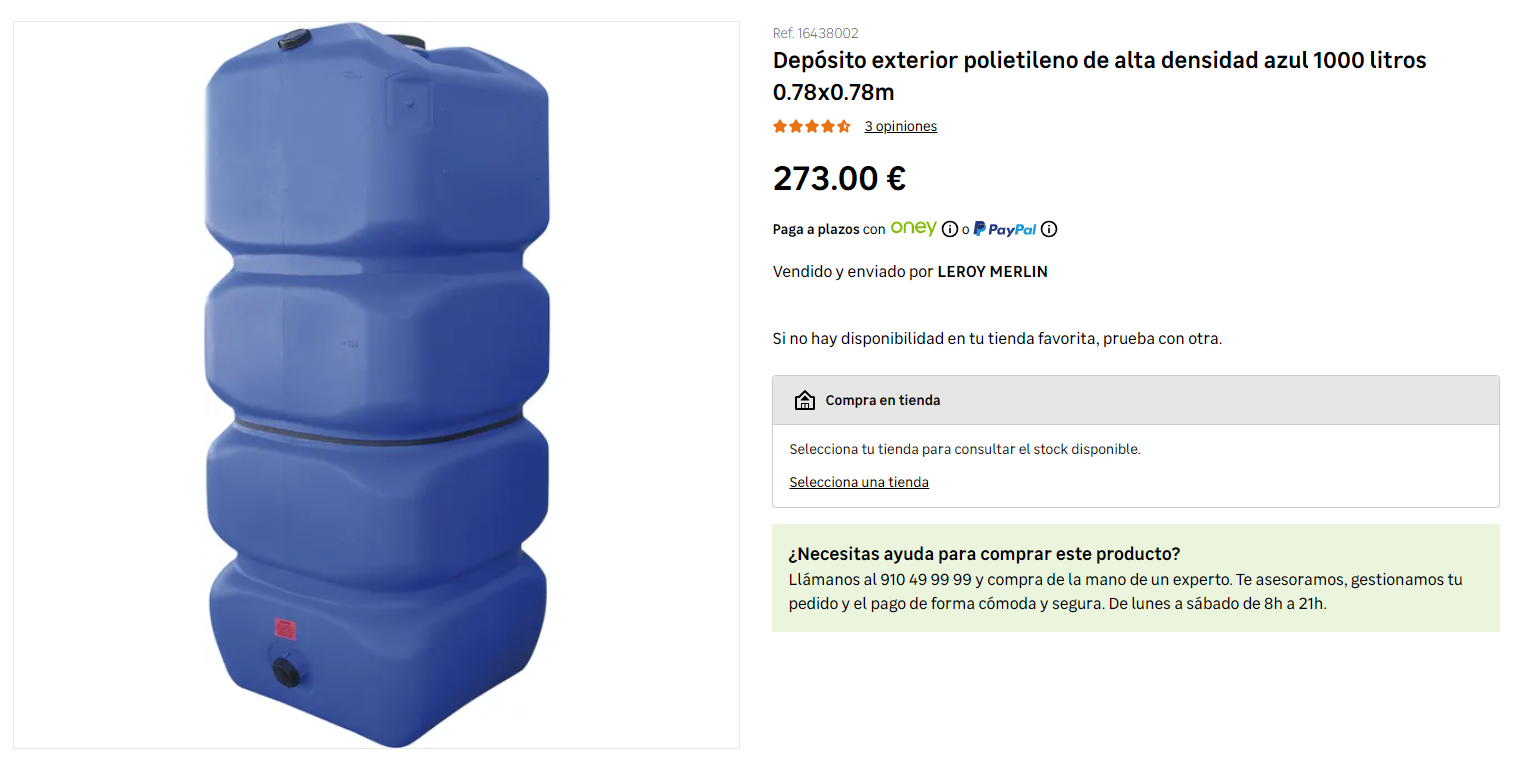
\includegraphics[width=0.5\linewidth]{Imagenes/DepositoAuxiliarAgua.png}
    \caption{Depósito auxiliar de alimentación.}
\end{figure}

\subsubsection{Cálculo de las bombas}
Siendo el caudal máximo simultáneo de la instalación de $0,85 dm^3/s$ y siendo este menor de $10 dm^3/s$ se necesitarán dos bombas, incluyendo la bomba de reserva. La presión mínima de arranque de estas bombas vendrá dado por la siguiente expresión:
\[Pb = Ha + Hg + Pc + Pr\]
donde
\begin{itemize}
    \item $Pb$: presión mínima de arranque
    \item $Ha$: altura geométrica de aspiración
    \item $Hg$: altura geométrica
    \item $Pc$: pérdida de carga del circuito 
    \item $Pr$: presión residual en el grifo, llave o fluxor
\end{itemize}
Se obtiene así una presión de arranque de $17,2252 mca$. Por lo que cada bomba deberá proporcionar por sí misma un caudal de $3,06 m^3/h$ con una altura de $17,2252 mca$. Se elige por tanto una bomba de presión de agua STERWINGS de 900 W de potencia con calderín de 24 litros. Que ofrece un caudal máximo de $3.800 l/h$ y una presión de $4,3 bar$. El coste de dicha bomba en Leroy Merlin se ilustra en la siguiente imagen:

\begin{figure}[H]
    \centering
    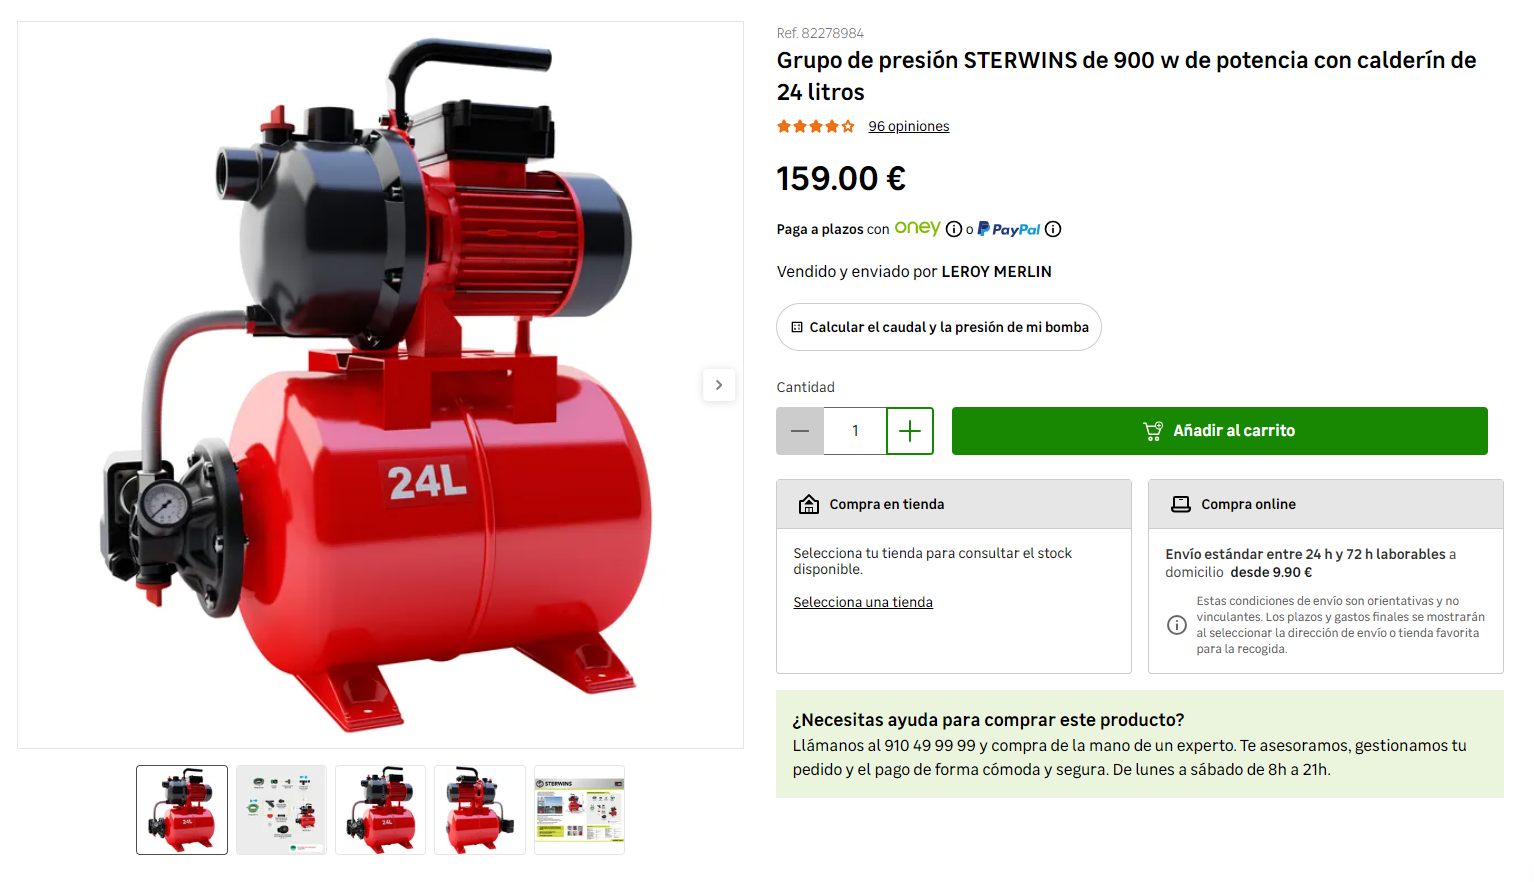
\includegraphics[width=0.5\linewidth]{Imagenes/BombaAgua.png}
    \caption{Bomba de presión de agua.}
\end{figure}

\subsubsection{Cálculo del depósito de presión}
El volumen del depósito vendrá dado por la siguiente expresión:
\[Vn = Pb \times \frac{Va}{Pa}\]
siendo
\begin{itemize}
    \item $Vn$: volumen útil del depósito de membrana
    \item $Pb$: presión absoluta mínima
    \item $Va$: volumen mínimo de agua
    \item $Pa$: presión absoluta máxima
\end{itemize}

Se obtiene así un volumen útil del depósito de membrana aproximado de $Vn = 11 L$, decidiendo optar por un vaso de expansión vertical multiusos Imera de $12 L$. El precio de dicho vaso de expansión en Amazon se ilustra en la siguiente imagen:
\begin{figure}[H]
    \centering
    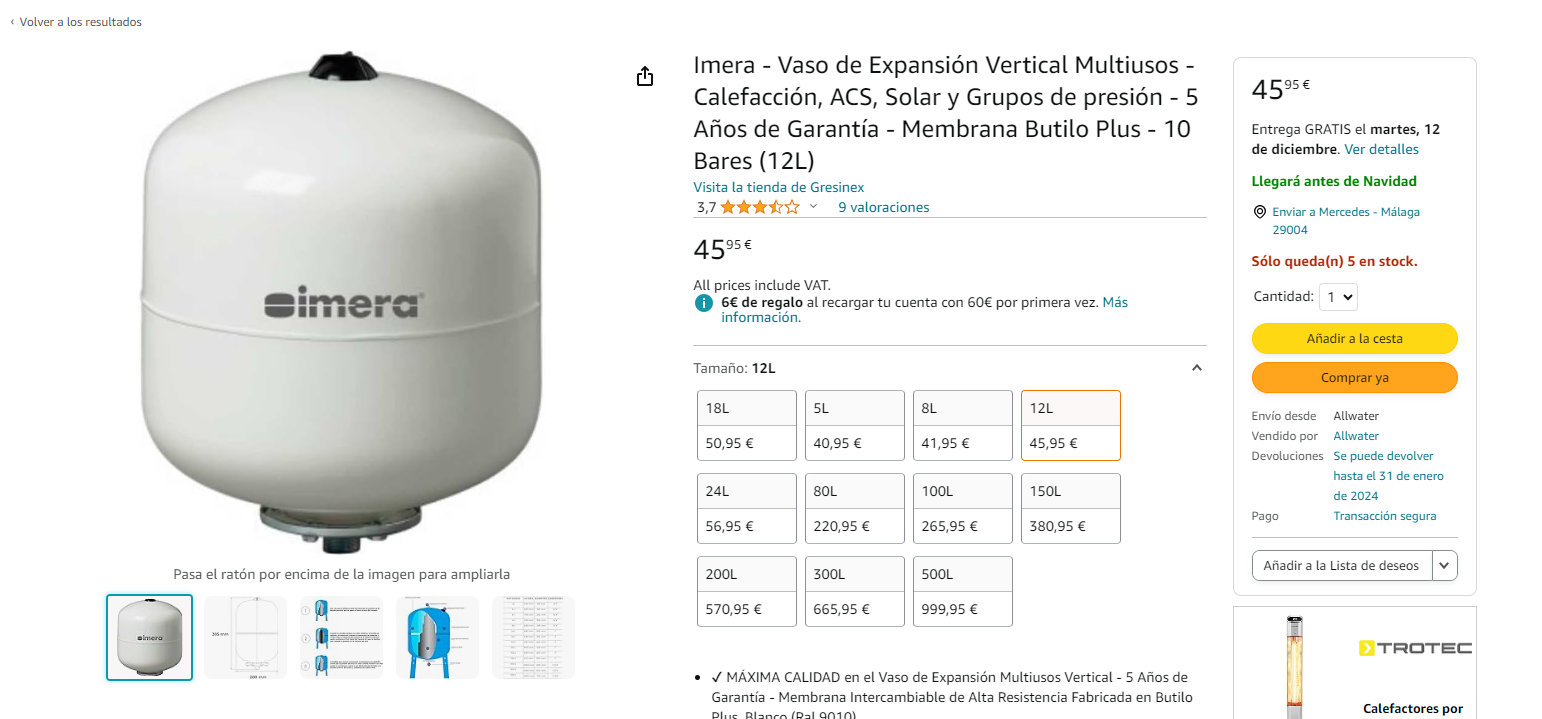
\includegraphics[width=0.5\linewidth]{Imagenes/Vaso de Expansion.png}
    \caption{Vaso de Expansión.}
\end{figure}

\subsection{Instalación de ACS}
El CTE HS-4 indica un consumo orientativo de ACS por persona para talleres, este es de $21 l$, por lo que para un taller como el del proyecto en el que habrá alrededor de 15 trabajadores, el consumo máximo diario de ACS será de:

\[Consumo_{max} = 15 \times 21 = 315 l\]

Aplicando un factor de utilización de $0,5$ a dicho consumo, se obtiene el volumen del acumulador de ACS necesario.

\[V_{acumulador} = 315 \times 0,5 = 157,5 l\]

Se decide instalar un termo eléctrico de $150 l$ que será suficiente para el abastecimiento de ACS para la nave. Dicho termo será el Bosch Termo eléctrico Tronic 6000T con una capacidad de 150 litros. El costo de dicho dispositivo en Bauhaus se ilustra en la siguiente imagen:

\begin{figure}[H]
    \centering
    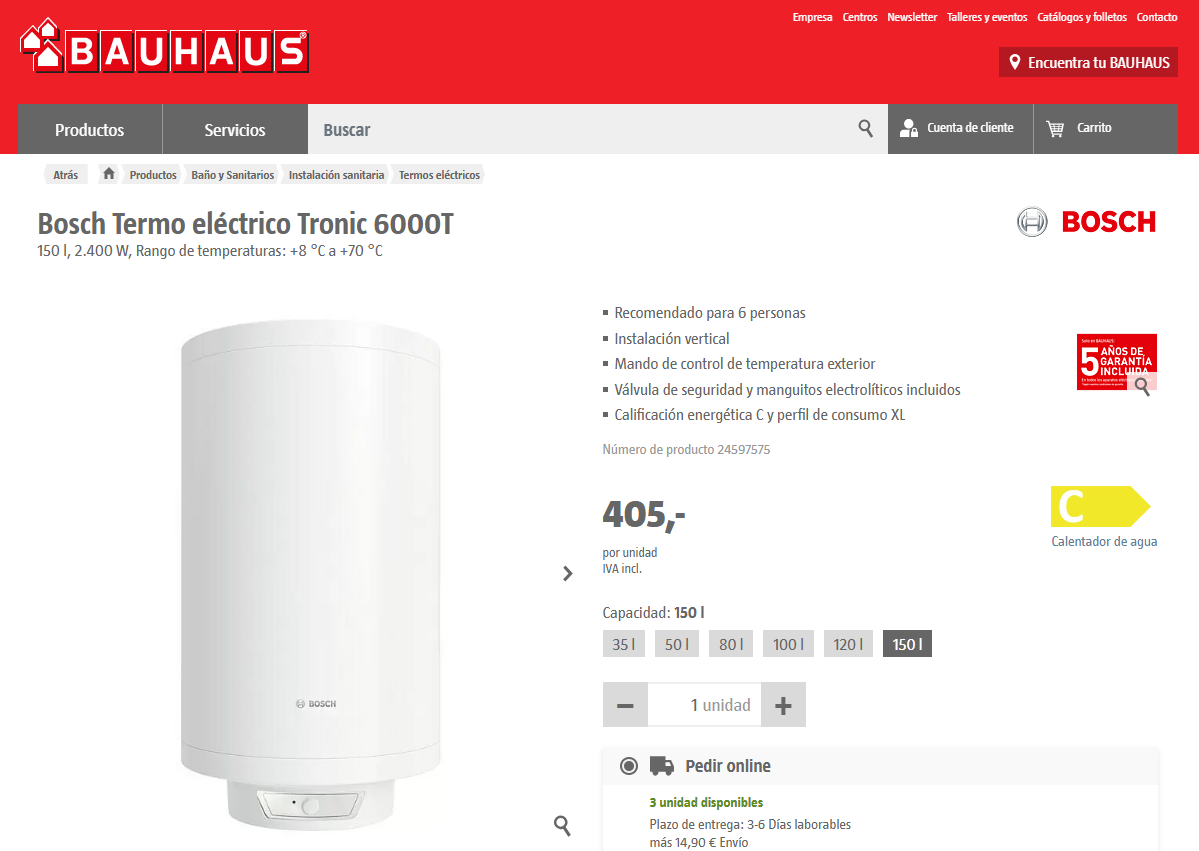
\includegraphics[width=0.5\linewidth]{Imagenes/Termo.png}
    \caption{Termo eléctrico seleccionado.}
\end{figure}

\end{document}